\documentclass[authoryear,preprint]{sigplanconf}

% The following \documentclass options may be useful:

% preprint      Remove this option only once the paper is in final form.
% 10pt          To set in 10-point type instead of 9-point.
% 11pt          To set in 11-point type instead of 9-point.
% authoryear    To obtain author/year citation style instead of numeric.

\usepackage{amsmath}

\usepackage{color}
\usepackage{MnSymbol}
\definecolor{light-gray}{gray}{0.94}
\usepackage{listings}
\lstloadlanguages{Haskell}
\lstnewenvironment{code}
    {\lstset{}%
      \csname lst@SetFirstLabel\endcsname}
    {\csname lst@SaveFirstLabel\endcsname}
    \lstset{
      basicstyle=\small\ttfamily,
      flexiblecolumns=false,
      frame=single,
      framerule=0.5em,
      rulecolor=\color{light-gray},
      %basewidth={0.5em,0.45em},
      showstringspaces=false,
      identifierstyle=,
      %%sensitive=true,
      breaklines=true,
      backgroundcolor=\color{light-gray},
      lineskip={-1.5pt},
      literate={/}{{$/$}}1 {*}{{$*$}}1
               {>}{{$>$}}1 {<}{{$<$}}1 {\\}{{$\lambda$}}1
               {\\\\}{{\char`\\\char`\\}}1
               {->}{{$\rightarrow$}}2 {>=}{{$\geq$}}2 {<-}{{$\leftarrow$}}2
               {<=}{{$\leq$}}2 {=>}{{$\Rightarrow$}}2
               {\ .\ }{{$\circ$}}2
               {>>}{{>>}}2 {>>=}{{>>=}}2
               {|}{{$\mid$}}1
               {~}{{$\sim$}}2
    }
% \lstset{prebreak=\raisebox{0ex}[0ex][0ex]
%        {\ensuremath{\rhookswarrow}}}
%\lstset{postbreak=\raisebox{0ex}[0ex][0ex]
%        {\ensuremath{\rcurvearrowse\space}}}
\lstset{breaklines=true, breakatwhitespace=true}

\usepackage{graphicx}
\usepackage{url}
\begin{document}

\special{papersize=8.5in,11in}
\setlength{\pdfpageheight}{\paperheight}
\setlength{\pdfpagewidth}{\paperwidth}

\conferenceinfo{FARM~'14}{September 6, 2014, Gothenburg, Sweden} 
\copyrightyear{2014}
\copyrightdata{978-1-4503-3039-8/14/09} 
\doi{2633638.2633647}

% Uncomment one of the following two, if you are not going for the 
% traditional copyright transfer agreement.

\exclusivelicense                % ACM gets exclusive license to publish, 
                                  % you retain copyright

%\permissiontopublish             % ACM gets nonexclusive license to publish
                                  % (paid open-access papers, 
                                  % short abstracts)

%\titlebanner{banner above paper title}        % These are ignored unless
%\preprintfooter{short description of paper}   % 'preprint' option specified.


\title{Making programming languages to dance to: Live Coding with Tidal}
%\subtitle{Subtitle Text, if any}

\authorinfo{Alex McLean}
           {Interdisciplinary Centre for Scientific Research in Music, University of Leeds}
           {a.mclean@leeds.ac.uk}

\maketitle

\begin{abstract}

Live coding of music has grown into a vibrant international community
of research and practice over the past decade, providing a new
research domain where computer science blends with the performing
arts. In this paper the domain of live coding is described, with focus
on the programming language design challenges involved, and the ways
in which a functional approach can meet those challenges. This leads
to the introduction of Tidal 0.4, a Domain Specific Language embedded
in Haskell. This is a substantial restructuring of Tidal, which now
represents musical pattern as functions from time to events, inspired
by Functional Reactive Programming.

\end{abstract}

\category{J.5}{Performing Arts}{}
\category{J.5}{Music}{}
\category{D.3.2}{Applicative (functional) languages}{}

\keywords
domain specific languages; live coding; music

\section{Introduction - Live programming languages for music}

\emph{Live coding} is where source code is edited and interpreted in
order to modify and control a running process. Over the past decade,
this technique has been increasingly used as a means of creating live,
improvised music \citep{Collins03a}, with new programming languages
and environments developed as end-user music interfaces
\citep[e.g.][]{Wang04, Sorensen05, Aaron11, McLean10c}. Live coding of
music and video is now a vibrant area of research, a core topic in
major Computer Music conferences, the subject of journal special
issues \cite{McLean14}, and the focus of international seminars
\citep{Blackwell14}. This research runs alongside emerging communities
of live coding practitioners, with international live coding music
festivals held in the UK, Germany and Mexico. Speculative, isolated
experiments by both researchers and practitioners have expanded,
developing into active communities of practice.

Live coding has predominantly emerged from digital performing arts and
related research contexts, but connects also with activities in
Software Engineering and Computer Science, under the developing
umbrella of live programming language research (see for example the
proceedings of the LIVE workshop, ICSE 2013). These intertwined
strands are revitalising ideas around liveness first developed decades
ago, explored in now well-established systems such as Self, SmallTalk,
Lisp, command line shells and indeed spreadsheets. Continuing this
tradition, and making programming languages ``more live'' is of
interest in terms of making programming easier to teach and learn,
making programs easier to debug, and allowing programmers to more
easily achieve creative flow \citep{Blackwell14}. How these different
strands weave together is not always clear, but cross-disciplinary
engagement is certainly warranted.

\section{Live coding as a design challenge}

Live coding of music brings particular pressures and opportunities to
programming language design.  To reiterate, this is where a programmer
writes code to generate music, where a running process continually
takes on changes to its code, without break in the musical output. The
archetypal situation has the programmer on stage, with their screen
projected so that the audience may see them work. This might be late
at night with a dancing nightclub audience \citep[e.g. at an
  algorave;][]{Collins14}, or during the day to a seated concert hall
audience \citep[e.g. performance by laptop ensemble;][]{Ogborn14}, or
in more collaborative, long form performance \citep[e.g. slow
  coding;][]{Hall07}. The performer may be joined by other live coders
or instrumental musicians, or perhaps even choreographers and dancers
\citep{Sicchio14}, but in any case the programmer will want to enter a
state of focused, creative flow and work beyond the pressures at hand.

There are different approaches to live coding music, but one common
approach is based on an improvised Jazz model. The music is not
composed in advance, instead the music is developed through live
interaction, with live coders `playing off' each other, or shaping the
music in sympathy with audience response. The improvisers might add
extra constraints, for example the live coding community in Mexico
City is known to celebrate the challenge of live coding a performance
from scratch, each of which lasts precious few minutes. ``Slow
coding'' is at the other end of the scale, exploring a more
conversational, meditative ethos \citep{Hall07}.

At this point it should be clear that live coding looks rather
different from mainstream software engineering. There is no time for
test driven development, little time to develop new abstractions, and
where the code is deleted at the end of a performance, there are no
long-term maintenance issues. However, live programming languages for
music do have strong design pressures. They need to be highly
expressive, both in terms of tersity, and also in terms of requiring
close domain mapping between the code and the music that is being
expressed. As music is a time-based art-form, representation of time
structures is key. Familiar mechanisms such as revision control may be
employed in unusual ways, supporting repeating structures such as
chorus and verse, where code is branched and merged within short
time frames, creating cyclic paths of development.

\subsection{Liveness and feedback}
\label{sec:feedback}
It is worth considering what we mean by the word \emph{live}. In
practice, the speed of communication is never instantaneous, and in
that sense nothing is completely live. Instead, let us consider
liveness in terms of \emph{live feedback loops}, where two agents
(human or computational) continually influence one another. We can
then identify different forms of liveness in terms of different
arrangements of feedback loops.

In a live coded performance, there are at least three main feedback
loops. One is between the programmer and their code; making a change,
and reading it in context alongside any syntactical errors or
warnings. This loop is known as \emph{manipulation feedback}
\citep{Nash11}, and may possibly include process and/or data
visualisation through debugging and other programmer tools. A second
feedback loop, known as \emph{performance feedback} \citep{Nash11},
connects the programmer and the program output, in this case music
carried by sound. In live coding of music, the feedback cycle of
software development is shared with that of musical development. The
third loop is between the programmer and their audience and/or
co-performers. We can call this feedback loop \emph{social feedback},
which is foregrounded at algorave events, where the audience is
dancing.  Together these feedback loops connect the programmer with
the live, passing moment.

% This relates to a yet another loop where peers act as
% critics, and give verbal feedback, in the case of live coding usually
% after a performance. \citet{dInvernoTODO} refers to this as
% \emph{creative feedback}, accentuating the role which social
% interaction has in what might otherwise be considered individual
% creativity.

%% This may involve including musical representation of time in the model
% of computation at play.
%  representing the particular musical styles under consideration, In
% the following we take these pressures in turn, introducing a
% declarative approach to describing music, and then extending that
% system into live interaction.

\subsection{Programming Language Paradigms for Music}

%Music takes many forms, and can be thought about and modelled in a
%multitude of different ways. In terms of adoption, the most successful
%digital representation is the venerable MIDI, which is based on a
%model of piano keyboard. However, MIDI relies upon a number of
%assumptions which do not always fit well, for example a clear
%distinction between composition and sound synthesis, and 14 bit
%parameter resolution. An alternative, in the present context of the
%FARM workshop, is to instead represent music with higher order
%constructs, written in domain specific languages designed for the
%purpose. The advantage of this approach is that the language can be
%based around rich time structures, and allow the music composer (or
%improviser) to define a relationship between time and sound that is
%particular to the piece \citep{@Collinge84}.

A large number of programming languages have been designed for
algorithmic music composition and digital sound processing (DSP) over
the past few decades, for example ChucK, SuperCollider, Max/MSP, HMSL,
Common Music and the MusicN languages. As processor frequencies have
increased, the promise of realtime processing has put new design
pressures on languages. Live coding has emerged over the past decade,
along with the promise of realtime programming as an exploratory
activity. This has been a social development as much as a
technological one -- although there have been breakthroughs, much of
the technology was already in place.

There are a range of programming language paradigms in computer
music. Perhaps the most dominant paradigm is dataflow programming;
declarative functions which do not return any values, but take streams
of data and inputs, and send streams of output to other functions as a
continual side effect. These languages, such as Max/MSP, PureData and
VVVV, usually have a graphical ``Patcher'' interface, where words are
contained within `boxes', connected with `wires' to form the dataflow
graph. The accessibility of these systems may be attributed to their
similarity to the analogue synthesisers which preceded and inspired
them \citep{Puckette88}.

The most common paradigm in live coding performance seems to
be functional programming; many live coding environments such as
Overtone, Fluxus and Extempore are Lisp dialects, and the pure
functional language Haskell is the basis of a number of live music
EDSLs (embedded domain specific languages); namely Conductive
\citep{Bell11}, Live-Sequencer \citep{Thielemann12} and Tidal. The
Tidal language is introduced in the following section, with emphasis
on its approach to the representation of time.

\section{Introducing Tidal}
\label{sec:intro}
% The author states that Tidal represents many years of development,
% and he has published before about Tidal. Something I miss is that
% the author does not clearly explain how the current version of Tidal
% differs from earlier versions he has published about. Clearly, an
% in-depth comparison is not necessary, but "several major rewrites"
% does not give me any information at all, and a bit more detail would
% be welcome.

Tidal represents many years of development, and the present paper
supersedes earlier work \citep{McLean10d}, with several major rewrites
since (\S \ref{tidaldev}). At its essence it is a domain specific
language for musical pattern, of the kind called for by
\citet{Spiegel81}, and present within many other systems including
HMSL, SuperCollider \citep{McCartney02} and ixilang
\citep{Magnusson11b}. Tidal has been developed through use, informed
by many dozens of high profile performances to diverse audiences, and
within diverse collaborations. The present author has predominantly
used it within algorithmic dance music \citep[algorave; ]{Collins14}
and improvised free Jazz performances \citep{Hession14}, as well as in
live art \citep{McLean12a} and choreographic \citep{McLean14}
collaborations. The software is available under a free/open source
license, and it now has a growing community of users (\S \ref{sec:community}).

Tidal is embedded in the Haskell language, taking advantage of its
rich type system. Patterns are represented using the below datatype,
which we will explain in the following.

\begin{center}
\begin{minipage}{0.5\textwidth}
\begin{lstlisting}
  type Time = Rational
  type Arc = (Time, Time)
  type Event a = (Arc, Arc, a)
  data Pattern a = Pattern (Arc -> [Event a])
\end{lstlisting}
\end{minipage}
\end{center}

\subsection{Representing Time}

In Tidal, time is rational, so that musical subdivisions may be stored
accurately as simple fractions, avoiding rounding errors associated
with floating point. Underlying this is the assumption that time is
structured in terms of rhythmic (or more correctly, metric)
\emph{cycles}, a perceptual phenomena that lies at the basis of a
great many musical traditions including Indian classical
\citep{Clayton08}, and electronic dance musics. The first beat of each
cycle, known as the \emph{sam}, is significant both for resolving the
previous cycle and for starting the next. The number line of whole
numbers represents successive sam beats.

The Tidal timeline can be conceptualised as a spiral, as Fig.
\ref{fig:spiral} illustrates; both repeating and progressing. Although
this is a cyclic structure, cycles will often change from one cycle to
the next. Indeed, polyrhythms are well supported in Tidal, but this
assumed cyclic structure acts as the metric anchor point for Tidal's
pattern operations.

% I do not understand the spiral nature of the timeline. Is it
% possible that the stop time of an arc is before its start time?

\begin{figure}[t]
    \centering
\includegraphics[width=0.45\textwidth]{images/spiral.pdf}
    \caption{The Tidal timeline as an infinite spiral, with each cycle represented as a natural number, which may be subdivided at any point as a rational number.}
    \label{fig:spiral}
\end{figure}

In practice, when it comes to turning a pattern into music, how cycles
relate to physical time depends on how fast the musician wants the
music to go. This is managed externally by a scheduler, and multiple
live coders can share a tempo clock over a network connection, so that
their cycles are locked in phase and frequency, and therefore playback
of their patterns is in time.

In sympathy with the focus on cycles, as opposed to the linear
progression of time, a time range is called an \lstinline{Arc},
specified with start and stop time. When an arc represents the
occurrence of a musical event, the start and stop are known as the
event \emph{onset} and \emph{offset}, which are standard terms
borrowed from music informatics.

% - section 3.1, pattern definition : the fact events are defined by
% - means of two Arcs (Time segments ?) seems very central but it is
% - hardly explained; pictures of pattern over a time line could make
% - it clearer ? are there some constraints generally satisfied
% - between these two Arcs ?

An \lstinline{Event} associates a value with two time arcs; the first
arc gives the onset and offset of the event, and the second gives the
'active' portion. The second arc is used for cases where an event is
cut into pieces; it is important for each piece to store its original
arc as context.

% the author states "The arcs of these events may overlap, in other
% words supporting musical polyphony". I wondered does this mean that
% the individual events are always monophonic? Would it not be possible
% to create a single event that performs a chord? If this is the case
% than polyphony indeed can only be created by overlapping (monophonic)
% events. However, if an events can contain harmony this phrase would
% just be false.

Finally, a \lstinline{Pattern} is represented as a function, from an
\lstinline{Arc} to a list of events. To retrieve events from the
pattern, it is queried with an \lstinline{Arc}, and all the events
active during the given time are returned. The arcs of these events
may overlap, in other words supporting musical \emph{polyphony}
without having to deal with events containing multiple values
(although Tidal events which contain chords rather than atomic events
are certainly possible).

All Tidal patterns are notionally infinite in length; they cycle
indefinitely, and can be queried for events at any point. Long-term
structure is certainly possible to represent, although Tidal's
development has been focused on live coding situations where such
structure is already provided by the live coder, who is continually
changing the pattern.

% a connection with Functional Reactive Programing (Elliot 2009) that
% could be made explicit by describing (recalling ?) the general
% architecture of Tidal.

This use of functions to represent time-varying values borrows ideas
from Functional Reactive Programming \citep{Elliott09}. However, the
particular use of time arcs appears to be novel, and allows both
continuous and discrete patterns to be represented within the same
datatype. For discrete patterns, events active during the given time
arc are returned. For continuous structures, an event value is sampled
with a granularity given by the duration of the \lstinline{Arc}. In
practice, this allows discrete and continuous patterns to be
straightforwardly combined, allowing expressive composition of music
through composition of functions.

\subsection{Building and combining patterns}

We will now look into how patterns are built and combined in
Tidal. Our focus in this section will be on implementation rather than
use, but this will hopefully provide some important insights into how
Tidal may be used.

Perhaps the simplest pattern is \lstinline{silence}, which returns no
events for any time:

\begin{center}
\begin{minipage}{0.5\textwidth}
\begin{lstlisting}
silence :: Pattern a
silence = Pattern $ const []
\end{lstlisting}
\end{minipage}
\end{center}

The `purest' discrete pattern is defined as one which contains a
single event with the given value, for the duration of each
cycle. Such a pattern may be constructed from a single value with the
\lstinline{pure} function, which Tidal defines as follows:

% May be you should explain the operator % of the non Haskell programmer.

\begin{center}
\begin{minipage}{0.5\textwidth}
\begin{lstlisting}
  pure x = 
    Pattern $ \(s, e) -> 
      map (\t -> ((t%1, (t+1)%1), 
                  (t%1, (t+1)%1),
                   x
                  )
                 )
                 [floor s .. ((ceiling e) - 1)]
\end{lstlisting}
\end{minipage}
\end{center}

This is an internal function which is not often used directly; we will
show alternative ways of constructing patterns later.

% Cat: The explanation was difficult to understand. Is it possible to
% give the code or at least the type signature?

Having constructed some patterns, we can combine them in different
ways. For example, the \lstinline{cat} function returns a pattern
which cycles through the given list of patterns over time. The
patterns are interlaced, i.e. taking the first cycle from each
pattern, then the second, and so on. To make this possible, the
resulting pattern needs to manipulate time values that are passed to
it, forward those values on to the patterns it encapsulates, and then
manipulate the time values of the events which are returned.

Although Tidal is designed for musical pattern, our example patterns
will be of colour, in sympathy with the current medium. The x axis
represents time travelling from left to right, and the y axis is used
to `stack up' events which co-occur. Here we visualise the first cycle
of a pattern, which interlaces pure blue, red and orange patterns:

<example>
cat [pure blue, pure red, pure orange]
</example>

% definition of density: What are the functions mapResultTime and mapQueryTime?
% section 3.2 : what are mapResultTime ? mapQueryTime ? does the
% author assume the reader to be familiar with Tidal
% implementation/architecture ?

We can use the \lstinline{density} combinator to squash, or `speed up'
the pattern so we can see more cycles within it:

<example>
density 4 $ cat [pure blue, pure red, pure orange]
</example>

Like \lstinline{cat}, density works by manipulating time both in terms
of the query and the resulting events. Here is its full definition,
along with its antonym \lstinline{slow}:

\begin{lstlisting}
density :: Time -> Pattern a -> Pattern a
density 0 p = p
density 1 p = p
density r p = 
  mapResultTime (/ r) (mapQueryTime (* r) p)

slow :: Time -> Pattern a -> Pattern a
slow 0 = id
slow t = density (1/t) 
\end{lstlisting}

% Time is represented with rational numbers and the density function
% allows putting several cycles of a pattern inside one cycle of
% another pattern. Therefore, is it possible to create a kind of Zeno
% effect where the end of a cycle is never reached due to an infinite
% number of patterns inside it?

The combinator \lstinline{slowcat} can be defined in terms of
\lstinline{cat} and \lstinline{slow}, so that the resulting pattern
steps through the patterns, cycle by cycle:

\begin{lstlisting}
slowcat :: [Pattern a] -> Pattern a
slowcat ps = 
  slow (fromIntegral $ length ps) $ cat ps
\end{lstlisting}

Now when we try to visualise the previous pattern using
\lstinline{slowcat} instead of \lstinline{cat}, we only see blue:

<example>
slowcat [pure blue, pure red, pure orange]
</example>

This is because we are only visualising the first cycle, the others
are still there.

The definition for combining patterns so that their events co-occur is
straightforward:

% definition of overlay: Instead of "The definition for combining patterns so that their events co- occur is straightforward", you can write something like "The definition for combining patterns so that their events co- occur is simply the union of their events".

\begin{center}
\begin{minipage}{0.5\textwidth}
\begin{lstlisting}
overlay :: Pattern a -> Pattern a -> Pattern a
overlay p p' = Pattern $ \a -> (arc p a) ++ (arc p' a)

stack :: [Pattern a] -> Pattern a
stack ps = foldr overlay silence ps
\end{lstlisting}
\end{minipage}
\end{center}

<example>
stack [pure blue, pure red, pure orange]
</example>

The vertical order of the events as visualised above is not
meaningful; that the events co-occur simply allow us to make
`polyphonic' music, where multiple events may sound at the same time.

By combining the functions we have seen so far, we may already begin
to compose some interesting patterns:

<example>
density 16 $ stack [pure blue,
                    cat [silence, 
                         cat [pure green, 
                              pure yellow]
                        ], 
                    pure orange]
</example>

\subsection{Parsing strings}

The functions we have defined so far for constructing patterns are
quite verbose, and therefore impractical. Considering that Tidal is
designed for live musical performance, the less typing the better. So,
a simple parser \lstinline{p} is provided by Tidal, for turning terse
strings into patterns, with syntax in part inspired by the Bol
Processor \citep{Bel01}. The previous colour pattern example may be
specified with this syntax as follows:

<example>
p "[blue, ~ [green yellow], orange]*16"
</example>

So, values within square brackets are combined over time with
\lstinline{cat}, and \lstinline{stacked} if they are separated by
commas. A pattern can have its density increased with
\lstinline{*}. Silence is specified by \lstinline{~}, analogous to a
musical \emph{rest}.

For additional tersity, the GHC string overloading feature is used, so
that the \lstinline{p} function does not need to be specified.

So far we have only shown the core representation of Tidal, but this
already allows us to specify fairly complex patterns with some tersity:

<example>
"[[black white]*32, [[yellow ~ pink]*3 purple]*5, [white black]*16]]*16"
</example>

If curly brackets rather than square brackets are used, subpatterns
are combined in a different way, timewise. The first subpattern still
takes up a single cycle, but other subpatterns on that level are
stretched or shrunk so that each immediate subelement within them are
the same length. For example compare the following two patterns:

<example>
density 6 $ "[red black, blue orange green]"
</example>

% Is it possible to give the implementation of the curly brackets?

<example>
density 6 $ "{red black, blue orange green}"
</example>

In musical terms, the first example would be described as a triplet,
and the latter a polyrhythm.

\subsection{Patterns as functors}

It is useful to be able to operate upon all event values within a
pattern irrespective of their temporal position and duration. Within
the functional paradigm, this requires the pattern datatype to be
defined as a functor. Because Haskell already defines functions and
lists as functors, defining \lstinline{Pattern} as a
\lstinline{Functor} instance is straightforward:

\begin{center}
\begin{minipage}{0.5\textwidth}
\begin{lstlisting}
instance Functor Pattern where
  fmap f (Pattern a) = 
    Pattern $ fmap (fmap (mapThd f)) a
  where mapThd f (x,y,z) = (x,y,f z)
\end{lstlisting}
\end{minipage}
\end{center}

This already makes certain pattern transformations trivial. For
example, musical transposition (increasing or decreasing all musical
note values) may be defined in terms of addition:

\begin{center}
\begin{minipage}{0.5\textwidth}
\begin{lstlisting}
transpose :: (Num a) => a -> Pattern a 
    -> Pattern a
transpose n pattern = fmap (+n) pattern
\end{lstlisting}
\end{minipage}
\end{center}

The \lstinline{Applicative} functor is a little more complex, but
allows a pattern of values to be mapped over a pattern of functions. A
minimal definition of Applicative requires \lstinline{pure}, which we
have already seen, along with the \lstinline{<*>} operator:

\begin{center}
\begin{minipage}{0.5\textwidth}
\begin{lstlisting}
(Pattern fs) <*> (Pattern xs) = 
  Pattern $ \a -> concatMap applyX (fs a)
  where applyX ((s,e), (s', e'), f) = 
     map (\(_, _, x) -> ((s,e), (s', e'), f x)) 
         (filter 
          (\(_, a', _) -> isIn a' s)
          (xs (s',e'))
         )
\end{lstlisting}
\end{minipage}
\end{center}

In combination with \lstinline{<$>} (which is simply \lstinline{fmap}
but in operator form), the \lstinline{<*>} operator allows us to turn
a function that operates on values, into a combinator which operates
on patterns of values. For example, we can use the library function
\lstinline{blend}, which operates on two colours, as a combinator
which operates on two colour patterns:
% The type signature of blend would help to understand the code
<example>
blend 0.5 
  <$> "[blue orange, yellow grey]*16" 
  <*> "white blue black red"
</example>

In the above, the \lstinline{blend} function is only able to operate
on pairs of colours, but the applicative definition allows it to
operate on pairs of colours taken from `inside' the two patterns. It
does this by matching co-occurring events within the first pattern,
with those in the second one, in particular the events in the second
pattern with arcs which contain the onset of those in the first
pattern. For example in the following \lstinline{red} matches with the
onsets of \lstinline{black} and \lstinline{grey}, and
\lstinline{green} matches with the onset of \lstinline{white}, so we
end up with a pattern resulting from blends of the colour pairs (red,
black), (red, grey) and (green, white).

<example>
(blend 0.5 <$> "[black grey white]" 
           <*> "red green")
</example>

Notice that the resulting pattern will always maintain the `structure'
of the first pattern over time. However where an event in the left
hand pattern matches with multiple events in the right hand pattern,
the number of events within this structure will be multiplied. For example:

<example>
(blend 0.5 <$> "[black grey white]" <*> 
       "[red green, magenta yellow]")
</example>

\section{Transformations}

From this point, we will focus less on the implementation of Tidal,
and more on its use. Please refer to the source code for any
implementation details.

\paragraph{Reversal}

Symmetry is fundamental to pattern, and so reversal is a key operation
in pattern manipulation. Because Tidal represents a notionally
infinite timeline, reversing a whole pattern is not possible. However,
the notion of a cycle is core to Tidal, and reversing each cycle
within a pattern is relatively straightforward.

<example>
rev "blue grey orange"
</example>

\paragraph{every}

Reversing a pattern is not very interesting unless you contrast it
with the original, to create symmetries. To do this, we can use
\lstinline{every}, a higher order transformation which applies a given
pattern transformation every given number of cycles. The following
reverses every third cycle:

<example>
density 16 $ every 3 rev "blue grey orange"
</example>

\paragraph{whenmod}

is similar to every, but applies the transformation when the remainder
of the first parameter divided by cycle number is less than the second
parameter.

<example>
density 16 $ whenmod 6 3 rev "blue grey orange"
</example>

\paragraph{Shifting/turning patterns}

The \lstinline{<~} transformation shifts a pattern to the left, or in
cyclic terms, turns it anticlockwise. The \lstinline{~>} does the
opposite, shifting it to the left/clockwise. For example, to shift it
one third to the left every fourth repetition, we could do this:

<example>
density 16 $ every 4 ((1/3) <~) 
                     "blue grey purple"
</example>

% The shifting/turning patterns operator <~ takes as argument a
% constant defining how the pattern must rotate. What happens if this
% constant is not a multiple of the pattern size? Is there an error at
% runtime? And more generally how errors are handled?

The above shows every fourth cycle (starting with the first one) being
shifted to the left, by a third of a cycle.

\paragraph{iter}

The \lstinline{iter} transformation is related to \lstinline{<~}, but
the shift is compounded until the cycle gets back to its starting
position. The number of steps that this takes place over is given as a
parameter. The shift amount is therefore one divided by the given
number of steps, which in the below example is \textonequarter{}.

<example>
density 4 $ iter 4 $ 
    "blue green purple orange"
</example>

\paragraph{superimpose}

is another higher order transformation, which combines the given
pattern with the result of the given transformation. For example, we
can use this with the transformation in the above example:

<example>
density 4 $ superimpose (iter 4) $ "blue green purple orange"
</example>

\paragraph{Combining transformations}

All of these pattern transformations simply return another pattern,
and so we can compose transformations together to quickly create
complex patterns. Because these transforms operate on patterns as
functions, and not simply lists, this can be done to arbitrary depth
without worrying about storage; no actual events get calculated and
manipulated until they are needed. Here is a simple example:

<examplegrid>
whenmod 8 4 (slow 4) $ every 2 ((1/2) <~) $
  every 3 (density 4) $ iter 4 
    "grey darkgrey green black"
</examplegrid>

To visualise some of the repeating structure, the above image shows a
ten-by-twenty grid of cycles, scanning across and down.

\section{Working with sound}

% The live coding aspect disappointed me. The introduction discusses
% live coding but not the rest of the paper. In particular, it does not
% discuss incremental definitions, and how to stop or modify a program
% being executed. These points are for me some key aspects of live
% coding. There are also just a few lines on how the logical time of
% Tidal matches the physical time during the performance.

The visual examples only work up to a point, and the multidimensional
nature of timbre is difficult to get across with colour alone. In the
case of Tidal, this multidimensional nature is evident in that
patterns of synthesiser parameters are defined, and combined into
patterns of synthesiser messages. In this way different aspects of
sound can be patterned into music independently, potentially creating
polyrhythmic structure that plays across different aspects of sound.

Tidal allows many aspects of sound, such formant filters,
spatialisation, pitch, onset and offset to be patterned separately,
and then composed into patterns of synthesiser control
messages. Pattern transforms can then manipulate multiple aspects of
sound at once; for example the \lstinline{jux} transform works
similarly to \lstinline{superimpose}, but the original pattern is
panned to the left speaker, and the transformed pattern to the
right. The \lstinline{striate} pattern effectively cuts a sample into
multiple `sound grains', so that those patterns of grains can then be
manipulated with further transforms. For details, please refer to the
Tidal documentation, and also to the numerous video examples linked to
from the homepage \url{http://yaxu.org/tidal}.

% TODO - examples

\section{Developing representation}
\label{tidaldev}

As stated earlier (\S \ref{sec:intro}), Tidal has progressed through a
number of rewrites, with major changes to the core representation of
pattern. By request of a peer reviewer, here we look at this
development of pattern representation over time. Each was motivated by
and informally evaluated through live performance.

The first representation was based on a straightforward tree
structure, where sounds could be sequenced within cycles, and layered
up as ``polymetries'', co-occuring sequences with potentially
different meters.

\begin{lstlisting}
data Event = Sound String
     | Silence
data Structure = Atom Event
     | Cycle [Structure]
     | Polymetry [Structure]
\end{lstlisting}

Haskell's default lazy behaviour allowed patterns to be represented of
infinite length, but not with random access - if one pattern is
replaced with another, either the event generation would restart from
the first event, or the whole performance up to the point of change
would have to be regenerated.

Next, a more functional approach was taken, representing pattern as a
function from discrete time to events, along with the period of the
cycle.

\begin{lstlisting}
data Pattern a =
  Pattern {at :: Int -> [a], period :: Int}
\end{lstlisting}

This was the basis of an earlier publication \citep{McLean10d}, and
worked reasonably well for particular styles of electronic dance
music, such as forms of acid house born from the step
sequencer. However, the discrete nature of time made it less suitable for
other genres, such as free jazz. This was worked around to some extent
by allowing a pattern of floating point time offsets to be applied,
but this did not allow for compound meters and other musical
structures.

Next a tree structure was returned to, but where cycles could contain
arcs, which had floating point onset and duration, allowing a freer
approach to time. The functional approach was preserved in the
\lstinline{Signal} data constructor, but for \emph{continuous}
patterns which continuously vary, rather than having discrete events
which begin and end.

\begin{lstlisting}
data Pattern a = Atom {event :: a}
               | Arc {pattern :: Pattern a,
                      onset :: Double,
                      duration :: Maybe Double
                     }
               | Cycle {patterns :: [Pattern a]}
               | Signal {at :: Double -> Pattern a}
\end{lstlisting}

Next, a simplification brought by the realisation that discrete
patterns could also be represented as functions from time ranges to
events:

\begin{lstlisting}
data Pattern a = Sequence {arc :: Range -> [Event a]}
               | Signal {at :: Rational -> [a]}
type Event a = (Range, a)
type Range = (Rational, Rational)
\end{lstlisting}

This worked well, particularly the use of rational numbers to
represent musical time. However, trying to deal with these quite
different forms as equivalent caused great complexities in the
supporting code. The final insight, leading to the present
representation (shown in \S \ref{sec:intro}), is that both discrete
sequences and continuous signals could be represented as the same
type, simply by sampling the midpoint of a range in the latter case.

\section{The Tidal community}
\label{sec:community}
% In general, I find user studies that investigate the to the
% usefulness of a language like Tidal a very valuable additions to
% these kind of papers. However, the survey presented in 6 has very
% little scientific value, and I think it was added to the paper for
% illustrative rather than scientific purposes. The number of
% respondents is very small, and it is unclear where the users come
% from exactly. The author only mentions "the Tidal on-line forum" as
% source.

Over the past year, a community of Tidal users has started to
grow. This followed a residency in Hangar Barcelona, during which the
Tidal installation procedure was improved and documented. This
community was surveyed, by invitation via the Tidal on-line forum
(\url{http://lurk.org/groups/tidal}), encouraged to give honest
answers, and fifteen responded. Two demographic questions were
asked. Given an optional free text question ``What is your gender?'',
10 identified as male, and the remainder chose not to answer. Given an
optional question ``What is your age?'', 7 chose ``17-25'', 4 chose
``26-40'', and the remainder chose not to answer.

Respondents were asked to estimate the number of hours they had used
Tidal. Answers ranged from 2 to 300, with a mean of 44.2 and a
standard deviation of 80.8. We can say that all had at least played
around with it for over an hour, and that many had invested
significant time in learning it; the mode was 8 hours.

A surprising finding was that respondents generally had little or no
experience of functional programming languages before trying
Tidal. When asked the question ``How much experience of functional
programming languages (e.g. Haskell, Lisp, etc) did you have when you
started with Tidal?'', 6/15 selected ``No experience at all'', 6/15
selected ``Some understanding, but no real practical experience'' and
3/15 selected ``Had written programs using functional programming
techniques''. \emph{No} respondents said that they had ``In depth,
practical knowledge of functional programming''.

Despite the general lack of experience with functional languages,
respondents generally reported that they could make music with Tidal
(14/15), that it was not difficult to learn (11/15), and that it had
the potential to help them be more creative (13/15). Furthermore, most
said they could learn Tidal just by playing with it (10/15), and that
they didn't need theoretical understanding in order to use it for
music (8/15). These answers were all captured as Likert responses, see
Figure \ref{fig:likert}. From this we conclude that despite Haskell's
reputation for difficulty, these users did not seem to have problems
learning a DSL embedded within it, that uses some advanced Haskell
features.

\begin{figure*}[t]
    \centering
    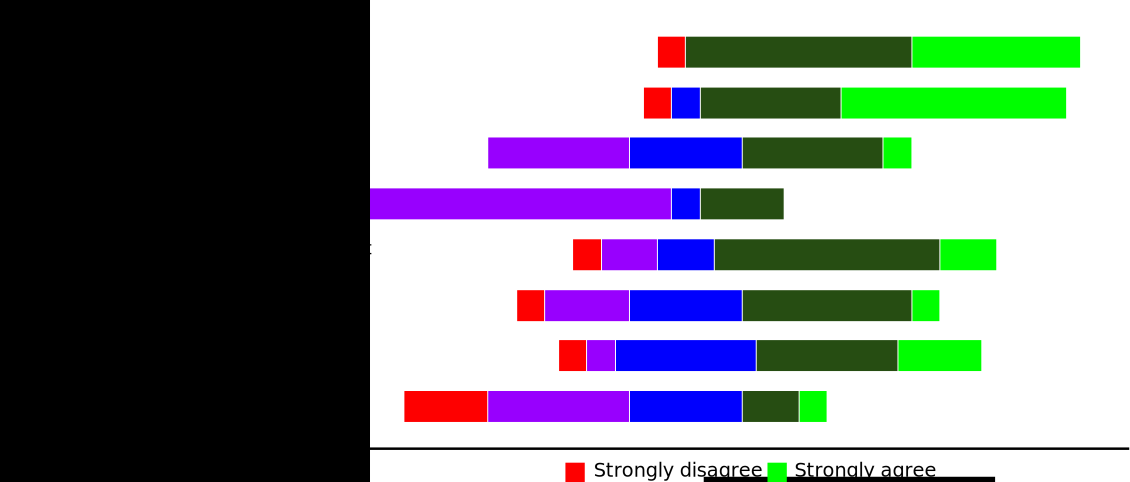
\includegraphics[width=0.95\textwidth]{images/graph.pdf}
    \caption{Likert scale questions from survey of Tidal users}
    \label{fig:likert}
\end{figure*}

This is very much a self-selecting group, attracted by what may be
seen as a niche, technological way to make music. Assessing
statistical significance is therefore difficult, but having learnt a
little about the background of respondents, we can turn to their
qualitative responses. These were in response to the free text
question ``In general, what has your experience of using Tidal been
like so far?'', and were overwhelmingly positive, to the point that
little critical reflection was offered. An interesting aspect though
is the extent to which respondents explained their experience of Tidal
in relation both to music software as well as programming languages.

\begin{quotation}
Respondent 1 (R1). Oddly it's the only time I've tried Haskell and
seen any point in Haskell over other languages I've played with.  I
think by starting as a sample player you've immediately brought
something like the 808 (or rebirth, or hydrogen in the linux world) to
text files.
\end{quotation}

\begin{quotation} R8. Tidal is the first music programming or
algorithmic music thingy I've tried which makes sense to me as a
musician (they all make sense to me as a coder). It's an instrument
that motivates me to learn and discover my sound within its
capabilities, a unique piece of gear.
\end{quotation}

Others responded in terms of the creative change that using Tidal has
signalled.

\begin{quotation}R10. Tidal has a therapeutic value for me which stems from its
immediacy and the fact that I can modify patterns at run-time and hear
the results instantly. It means I find myself 'in the zone' or in a
state of 'flow'. It's akin to jamming through programming.
\end{quotation}

\begin{quotation}
R12. Tidal has made a vast difference to my creative life - I didn't
write music for 10 years after Fruityloops became FL Studio with a
more audio oriented approach (rather than just being a solid pattern
programmer) and could no longer figure out how to put my more complex
ideas to disk. Now I've recorded a couple hours' worth of music in
under six months which, in itself, is amazing to me.
\end{quotation}

\begin{quotation}
R15. I'm loving it. It's a great way in to functional programming, and
the pattern syntax has changed how I think about digital
representations of music
\end{quotation}

The Tidal user community remains small -- there are currently 56
members of the online forum, and 164 'stars' and 24 forks on github,
and so it is difficult to generalise from these survey
results. However, it is encouraging that respondents report such
positive experiences despite lack of background in functional
programming, and future work is planned to bring out this reflection
using Interpretative Phenomenological Analysis
\citep[IPA;][]{Smith04}.

\section{Discussion}

We have given some context to live coding Tidal, described some
implementation details and a selection of the functionality it
provides. This functionality is strongly supported by Haskell itself, which
has proved to be a language well suited for describing pattern. This
is borne out from a small survey of 15 Tidal users, who generally
reported positive learning experiences despite not being experienced
functional programmers.

Programming while people are dancing to your code makes the abstract
tangible. It is necessary to achieve creative flow in performance,
particularly in the form of improvised performance common in live
coding practice. Flow is not a case of `losing yourself', but rather
optimal, fully engaged experience. To experience creative flow while
constructing abstract structure is something which perhaps all
programmers are familiar with and strive for, but to be in this state
while experiencing those abstract structures as sound,
together with a room full of people whose physical responses you are
both shaping and reacting to through the code, is a rare feeling. It
is not just about connecting with people, although that is a large
part of it. It is also the feeling of being \emph{in time}. Everything
counts, not only what you type, but when. The live coder needs to be
continually aware of the passing of time, so that the shift that comes
with the next evaluation fits with (or against) the expectations of
those listening or dancing to it.

Tidal fits within this process by being highly viscous and requiring
low cognitive load \citep{Green00}, therefore supporting playful
engagement and a high rate of change. The generality of the pattern
transformations means that live coders can apply a set of heuristics
for changing code at different levels of abstraction, as tacit
knowledge built through play. Live coding is a relatively young field,
and this tacit knowledge is still at early stages of development, as a
creative and social process. Perhaps most excitingly for FARM,
programming language design is part of this process.

\acks

Thanks and gratitude to the members of the Tidal community for their
feedback, suggestions and input into the ongoing development of Tidal.

\bibliographystyle{abbrvnat}

% The bibliography should be embedded for final submission.
%\begin{thebibliography}{}
%\softraggedright
%\bibitem[Smith et~al.(2009)Smith, Jones]{smith02}
%P. Q. Smith, and X. Y. Jones. ...reference text...
%\end{thebibliography}

\bibliography{alex}

\end{document}

% From the mailing list ..

% How are you deciding where to grow the language? Is this based, by
% and large, on your performance experiences? Or does it grow out of
% the patterns research? e.g.

% I'm reading in Pattern.hs now. Does it help you to explain how the
% timing is structured, in any additional detail?

% 1) Using a functional language, what are the benefits?
% 2) Does tidal view calling Dirt a "side-effect"
% 3) W/ your work on a visual tidal (with the pipes, forget what you called 
% it), have you thought of other visualizations (other than the awesome pdfs).
% 4) Is the sync part easy to dive into (that's the part I'd most like to
% mess with, to just get things synced to a midi clock)

